This chapter summarises the outcomes of two use cases conducted with the implemented prototype c3po and
the results. First the goals of the experiments and some general information about the content sets are defined. Then the two use case are summarised and some of the interesting results are presented. The first use case is conducted on rather heterogeneous content and the second one over a web archive.

\section{Goals and General Information}
In order to test and validate c3po a large set of files is to conduct experiments over them.
For this work we use two sets of data to conduct similar experiments on the same commodity machine. The number of objects in each set is in the order of hundreds of thousands objects with a upper border of one million. This volume is large enough to capture the requirements of many organisations and institutions. However, it is noteworthy, that there are institutions (such as Web Archives) with many millions and even billions of objects. Future work might focus on such use case studies.

The machine used for all the experiments (unless otherwise stated) is a common laptop with a 2.3 GHz Intel Core i5 Processor (2 Cores), 8 GB RAM and a common internal hard drive with 5400 rpm. As c3po is meant to run on a server it is very likely that this configuration is much less capable than the common server used within stake holding institutions, considering the current trend of hardware technology.

The authors hypothesis is that the processing power as well as the hard drive device would be the limiting factors during data gathering in the following experiments. The  processing of each file alone is a fast operation, however traversing the file system, opening and closing a stream to each file and storing the data to the local hard drive (within the database ) are relative expensive operations. Thus the disk write speed and the processing capacity are of a bigger importance. The RAM capacity will play an important role during analysis as the map-reduce jobs will strongly depend to that.

The goal of these use cases is to find out the usefulness of the tool in terms of speed, scalability of resources and volume of the data. Also the authors try to find out different filters with c3po in order to partition the file sets in meaningful homogeneous partitions and select representative sample objects for some of these sets.

% how is this going to be validated.

\section{GovDocs1}
DigitalCorpora.org\footnote{http://digitalcorpora.org} is a website that provides digital corpora for use in computer forensics education and research. The sites offers different file sets, network dumps, disk images and more. For the following experiments we use the GovDocs1 file set, which contains of nearly one million freely-redistributable files that resided in the .gov domain.
The files are randomly distributed into 1000 directories with up to 1000 files in each directory and can be downloaded at \url{http://digitalcorpora.org/corp/nps/files/govdocs1/}.

\subsection{Data Description}
Forensic Innovations Inc.\footnote{http://www.forensicinnovations.com/} have provided a simple statistical report that shows some of the important characteristics of the set, which we will try to find out with c3po and provide even more deeper insight. The report can be found here: \url{http://digitalcorpora.org/corpora/files/govdocs1-simple-statistical-report}. In table \ref{tab:govdoc1_general_info} general information such as file size and volume is summarised, whereas table \ref{tab:govdoc1_content} provides a summary over the content of the different files. Note that the total sum of files in the second table is more than the number of files in the set, meaning that many files are counted twice or even more, which is of course not very helpful for digital preservation activities.

\begin{table}
\centering
\begin{tabular}{l || c }
\hline
Characteristic & Total \\
\hline
\hline
Nr. Files & 986278 \\
File Size (KB) & 488658258 \\
Wrong File Extension & 33917 \\
Scan Time & 10:12:37 \\
\hline
\end{tabular}
\caption{This table shows the general information of the GovDocs1 data set.}
\label{tab:govdoc1_general_info}
\end{table}

\begin{table}
\centering
\begin{tabular}{l || l }
\hline
Content & Total \\
\hline
\hline
  Personal/User Data & 961914\\
  Text & 727217 \\
  Document & 539100 \\
  Hypertext & 467405 \\
  Graphic Image & 464870 \\
  Macro/Script &    351781 \\
  Font & 231275 \\
  Spreadsheet & 85110\\
  Program Data  &      41616\\
  Source Code & 36580 \\
  Raw Printer Data &  26190 \\
  Database & 24820 \\
  Archived Files & 14093 \\
  Video &  3483 \\
  Email & 2007 \\
  N/A  & 882 \\
  Template & 306\\
  Program Executable & 277\\
  Presentation & 222 \\
  CAD/3D Model & 138 \\
  Game Data &15\\
  Sound/Audio & 10 \\
  Shortcut/Link & 5 \\
  Library of Functions & 2\\
  Form & 2 \\
  Encryption Key  & 1\\
\hline
\end{tabular}
\label{tab:govdoc1_content}
\caption{This table shows the different content types within the GovDocs1 set as the preliminary data shows.}
\end{table}

\subsection{Experiment Preparation}
In order to conduct the experiment all the files have to be characterised with the FITS tool. In order to automate this task, the authors have used a workflow engine developed by the University of Manchester called Taverna\footnote{http://www.taverna.org.uk/}. With the help of Taverna, one can create parallelised workflows that consist of number of small steps and tasks. In this instance, the files were copied via \textit{scp} from a storage server, \textit{FITS} was executed in parallel on each of the files and the output was stored on the experiments machine.

Unfortunately, the current version of FITS (v0.6) was not stable for all file types and thus it was unable to produce output for some files. Thus all the experiments conducted on the set are done on a slightly smaller subset consisting of 945746 instead of 986278 files.

\textbf{\textit{Disclaimer}}: Due to the unpredictable behaviour of FITS on certain file types the workflow had to be restarted numerous times. Thus it was impossible to capture the real time for characterisation. In the following all times intervals that are given are only for the execution of c3po, unless otherwise noted. Thus any comparison with the scan time in the preliminary data should not be taken lightly. Nonetheless, the results provided here, shall give a good overview of what would be possible with a tool such as c3po.

\subsection{Experiment}
The actual experiment consists of number of steps. All these experiments were conducted with c3po v0.2.0 that can be downloaded from here (\url{https://github.com/peshkira/c3po/downloads}). 

First the data is gathered via c3po into a local instance of a Mongo Document store. The time for traversing the file system, parsing the data and storing it to the db is taken into account. The experiment is done with a single thread and with numerous threads to show the performance boost of the parallelisation.

In a next step some measurements are done for data export and profile generation, which will be important in a real world scenario.

In the last step of the experiment the gathered data is used and analysed with the c3po web application. Different characteristics and findings are presented as well as some measurement times of the map reduce jobs and further data. The tool is used to partition the content. At the end interesting data for some partitions is provided as well as their profiles.

\subsubsection{Gathering}
In the initial test the gathering was conducted in a single thread environment. 

\begin{verbatim}
c3po -g ~/path/to/folder/ -r -c govdocs1
\end{verbatim}

The processing of all 945746 files took more than 167 minutes. 47 files were not processed successfully due to malformed meta data files. After initial preparation and setup, processing 1000 files took 10.46 seconds on average.

The same procedure was conducted with 4 threads and with 8 threads. The speedup was 114 and 104 minutes respectively. The average processing of 1000 files was .. and .. respectively. This shows about 30\% increase in speed. More powerful hardware (with a solid state drive disk and faster CPU) will most probably enable a speedup up to 50\%. The next step could be to also parallelise the process on different nodes against the same DB.

\subsubsection{Profile \& Export}
In this part of the experiment c3po was used to generate a profile of the data processed in the previous step and to also export it. The generated files are then inspected.

\begin{verbatim}
c3po -p ~/path/to/output/folder -c govdocs1
\end{verbatim}

The time taken for the profile generation of the whole govdocs1 collection was 12 minutes. The profile included 112 properties. The output file was 53 KB in size, which is an acceptable size for transfer over the network.

The same command was then executed with the -ie switch, which includes the element identifiers in the profile.
The time taken was 12 minutes once again and the resulting file was 60 MB in size. This was due to the fact that all object identifiers were included in the profile. Since the collection is pretty big, this shows how infeasible this option is. It is helpful for demonstration purposes on smaller collections, but will not work in real world scenarios. This part of the profile should be swapped with a special query that selects the digital objects falling into this profile. This query should be understood by client and integrating applications, such planning tools and digital repositories. If this is the case, the footprint will be small and generation, as well as transfer over the network will be feasible.

%TODO include what was in the profile and some results.

\begin{verbatim}
c3po -e ~/path/to/output/folder -c govdocs1
\end{verbatim}
Afterwards all the data was exported to a .csv file in a sparse matrix, with the object identifiers as rows and the properties as columns. The generation took a little more than 2 minutes and resulted in a file of 430 MB in size. This matrix view is very helpful to obtain an overview of the whole collection and can be used to apply some more complex filters that are not possible with the web application. On the downside, it is questionable if this approach will scale for bigger collections. While state of the art spreadsheet processors still cope with files of this size, it is highly questionable if it will be possible to open a much larger file.

\subsubsection{Analysis}
The web app of c3po revealed that the whole collection of digital objects had an overall size of 447.36GB of data. This value seems to be realistic considering that FITS failed on numerous objects and the c3po gathering process failed on some as well. The smallest object has a size of 7 Bytes and the largest - 1.52GB. On average all of the objects have a size of 0.48 MB with a standard deviation of 4.29 MB.

C3PO immediately showed, that the collection consists of 46 different mime types and in addition there is one subset of conflicted mimes, which is the second most occurring. The first 9 most occurring mime types represent nearly 80\% of the whole collection and are presented in table \ref{tab:govdocs1_mimetypes}. The correlation between the mime type the format of a digital object implies that both distributions are similar. This was proven by c3po as well.

%APPENDIX?
%The whole distribution is presented in figure

\begin{table}[h]
\centering
\begin{tabular}{l || l }
\hline
Mime Type & Count \\
\hline
\hline
 application/pdf & 224495 \\
 conflicted 	& 160354 \\
 text/html		&  138161 \\
 image/jpeg	&  106714 \\
 text/plain		& 93280 \\
 application/mswod & 73282 \\
 application/vnd.ms-excel & 42877 \\
 image/gif		& 35292 \\
 text/xml		& 25347\\
 \hline
\end{tabular}
\caption{This table shows the 9 most occurring mime types within the GovDocs1 set as c3po showed.}
\label{tab:govdocs1_mimetypes}
\end{table}

The next interesting observation was the creation date distribution of the content set. The following table \ref{tab:govdocs1_created} presents it. The total of the files in this distribution is much less than the total of the collection, because of the data sparsity. Nonetheless, there are some interesting observations that can be made out of this distribution. Firstly, the objects created between 2003 and 2008 are much more than the rest. This can be related to the fact that data production does not increase constantly, but rather exponentially during the years. Although this conclusion might be biased as the data may not be sufficient to back it up. Secondly, it is very interesting that the data created in 2009 is  less than some data created during the 90s. Thirdly, there is one small subset that is gathered in year '-1'. This is clearly a faulty measurement provided by some of the characterisation tools bundled in FITS, which proves the point of the importance of meta data quality. 
Last but not least, there is one subset that seems to be created in 1910, which seems to be rather peculiar and might also be related to bad data quality.

\begin{table}[h]
\centering
\begin{tabular}{l || l }
\hline
Created Date & Count \\
\hline
\hline
2004 	& 38246 \\
2007 	&  37526 \\
2008		&  37152 \\
2006 	&  36276 \\
2005		&  35780 \\
2003		&  35204 \\
2002		&  26327 \\
2001		&  20134 \\
2000		& 15976 \\
1999		& 13006 \\
1998		&  9334 \\
1997		&  5597 \\
2009		&  5357\\
1996		&  2725\\
-1		&  2703\\
1910		&  2052\\
Rest		&  6362\\
 \hline
\end{tabular}
\caption{This table shows the 9 most occurring mime types within the GovDocs1 set as c3po showed.}
\label{tab:govdocs1_created}
\end{table}

%\begin{figure}[t]
%\begin{center}
%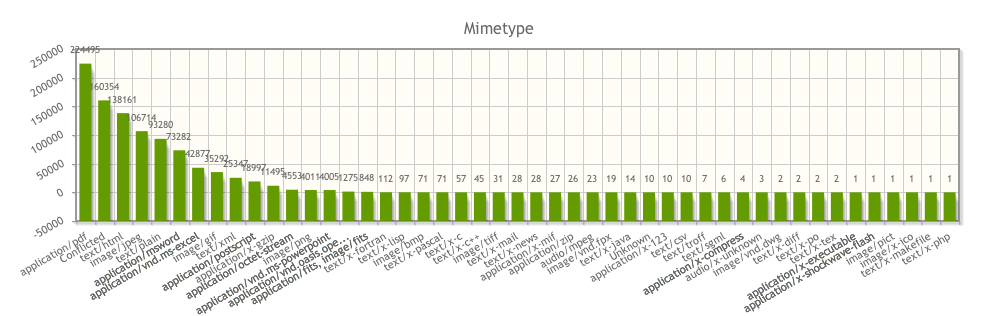
\includegraphics[width=\textwidth]{figures/usecases/govdocs1/govdocs1_mimetypes.png}
%\caption{All occurring mime types in govdocs1.}
%\label{fig:govdocs1_mimetypes}
%\end{center}
%\end{figure}



\section{Web Archive}